% !TeX root = ../main.tex
% -*- coding: utf-8 -*-

\chapter{仿真实验与评估}

我们选择一种简单的民间纸牌游戏,来验证前面所提出的强化学习理论是否能够较为适应地处理现实中的实际问题。

\section{实验环境建立}

\subsection{纸牌游戏的背景与规则介绍}

在本游戏中,初始牌面会去掉 “红桃2”、“梅花2”、“方块2”、“黑桃A”这 4 张牌,共计 48 张牌,每人发牌 16 张。第一回合由持手牌“黑桃3”的玩家出牌,随后依逆时针顺序跟牌,且要求在能出牌的情况下必须出牌,不可直接过牌。

作为第一位玩家出牌时,可任意选择牌型出牌,而跟牌阶段则只能按规则在指定牌型下出牌。该游戏规则简单,共有以下几种牌型:

\begin{center}
    \tablecaption{牌型介绍}
\begin{tabular}{|c|c|c|c|}
    \hline
    牌型简称 & 牌型描述 & 牌型简称 & 牌型描述 \\
    \hline
    对子 & 两张相同的牌 & 三条 & 三张相同的牌 \\
    \hline
    炸弹 & 四张相同牌 & 三带一 & 三条+单牌 \\
    \hline
    三带二 & 三条+任意两张牌 & 单顺 & 至少5张的连续牌 \\
    \hline
    双顺 & 至少2组连续对子 & 三顺 & 至少2组连续三条 \\
    \hline
    飞机 & 至少2组连续三带二 & 四带二 & 炸弹+任意两张牌\\
    \hline
\end{tabular}

\end{center}

最先将手牌出完的玩家为胜者。

\subsection{模拟建立的纸牌游戏环境}

基于游戏的基本规则,使用 \texttt{Python} 编程语言构建了一个简单的游戏模拟环境。为了能够进行数值化的模型训练,需要将不同纸牌转化为对应的数值编号,具体地,将游戏规则下一副牌(该规则下共 48 张牌)从 “黑桃3” 到 “方块2” 由小到大对应为一个长度为 48 的一维向量,每张牌都有一个唯一的 ID ,例如 \texttt{['黑桃3', '黑桃5', '红桃5', '梅花5', '黑桃7']} 转化后应为 \texttt{[0, 8, 9, 10, 16]}。后面的实验介绍中,模型内部结构均基于此前提。

在 \texttt{utils.py} 文件中,定义了 \texttt{divide\_cards()} 函数来实现发牌功能,能够随机将 48 张牌分为三份,发放给三位玩家,每位玩家各自分配到长度为 16 的一维向量,代表自己的手牌。

同时还定义了 \texttt{calculate\_score()} 函数,它能够根据游戏规则来计分,起到向模型传递反馈奖励值的作用。

在 \texttt{RunFastGame.py} 中,定义了一个完整的 \texttt{RunFastGameEnv} 类,它能够完整地模拟卡牌游戏对局,其中 \texttt{RunFastGameEnv.get\_state()} 函数能够获得当前所处的状态,\texttt{RunFastGameEnv.play\_cards()} 能够接收策略传入的指令来采取相应的行动。

具体地,\texttt{RunFastGameEnv} 能够模拟卡牌游戏对局中的每位玩家,它能基于环境信息以及模型的策略决策情况来模拟完整的游戏对局,从而产生了真实的经验数据,提供给模型进行 Monte Carlo 模拟,从而得以实现之前提出的算法。

\section{算法仿真与评估}

\subsection{Deep Q-Network 算法实现细节}

在 \texttt{DQN.py} 中,定义一个 \texttt{QNet} 类,建立一个全连接神经网络,其深度为 3 层。Input layer 有 209 个神经元,对应输入特征向量的 209 个元素;Hidden layer 1 有 512 个神经元;Hidden layer 2 有 256 个神经元;Hidden layer 3 有 128 个神经元;Output layer 只有一个神经元,其输出值为 $Q$ 函数所对应的值,如下图所示。

\begin{figure}[H]
    \centering
    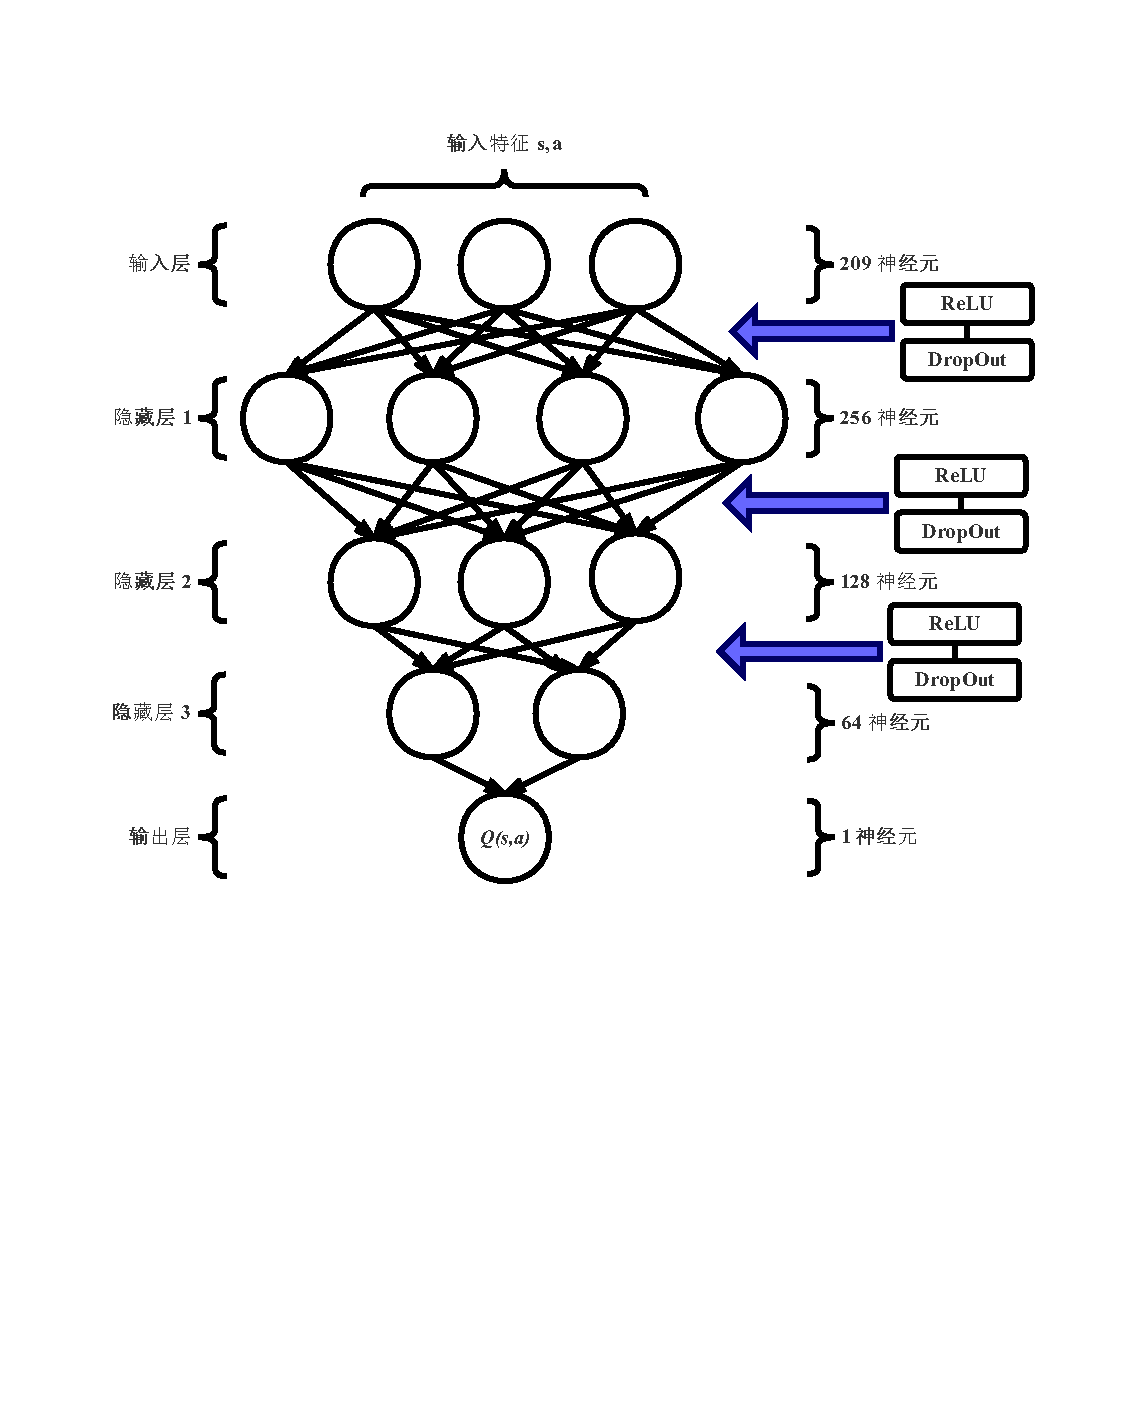
\includegraphics[width=\textwidth]{DQN-Detail.pdf}
    \caption{Deep Q-Network 实现细节}
\end{figure}

此外还定义了一个 \texttt{DQN} 类,用来实现 Deep Q-Network 的细节。其中,\texttt{DQN.choose\_action()} 函数代表策略函数 $\pi$ ,其功能是根据输入的状态 $s$ ,根据通过 $Q$ 函数大小决定的策略概率分布 $\pi(a|s)$ 来决定下一步应采取的行动 $a$ ;\texttt{DQN.store\_transition()} 函数和 \texttt{DQN.add\_reward()} 函数用于将模拟过程中的一些关键信息存储于记忆池中;\texttt{DQN.learn()} 函数的作用是将记忆池的信息提取出来,通过神经网络进行 Q-Learning 更新,更新公式为

\begin{equation}
    Q(S_t,A_t)\leftarrow Q(S_t,A_t)+\alpha\left[R_{t+1}+\gamma  \max\limits_aQ(S_{t+1},a)-Q(S_t,A_t)\right]
\end{equation}

最后,将 Deep Q-Network 模型接入进前面构建好的 \texttt{RunFastGameEnv} 环境下,即可开始模拟和训练的过程。

\subsection{仿真实验流程}

基于前面所描述的细节,本实验的具体流程如下:

\begin{algorithm}[H]
    \caption{训练过程}
    \begin{algorithmic}[1] %每行不显示行号
        \State 初始化三名不同的玩家 $A, B, C$
        \Repeat
        \State 开始新一局游戏,并为三名玩家发牌
        \Repeat
        \State 根据游戏规则决定当前回合应当出牌的玩家
        \State 进入当前玩家的视角,根据场面信息获取当前所处状态 $S$
        \State 将状态 $S$ 传入 $Q$ 函数 和 $\pi$ 策略,决策下一步所要采取的行动 $a$
        \State 实际采取行动 $a$ ,接收环境传递的反馈值,并存入记忆池
        \Until{执行行动 $a$ 后本局游戏分出胜负}
        \State 根据游戏规则,统计该局游戏各玩家得分,并追加存储至记忆池
        \State 将记忆池的信息,作为输入参数传入神经网络
        \State 经由神经网络完成一次训练学习,得到新的 $Q$ 函数和 $\pi$ 策略,用于下一次决策
        \Until{达到预设的训练次数}
        \State 结束训练,输出训练所得到的模型和参数
    \end{algorithmic}
\end{algorithm}

实验的流程图如下:

\begin{figure}[H]
    \centering
    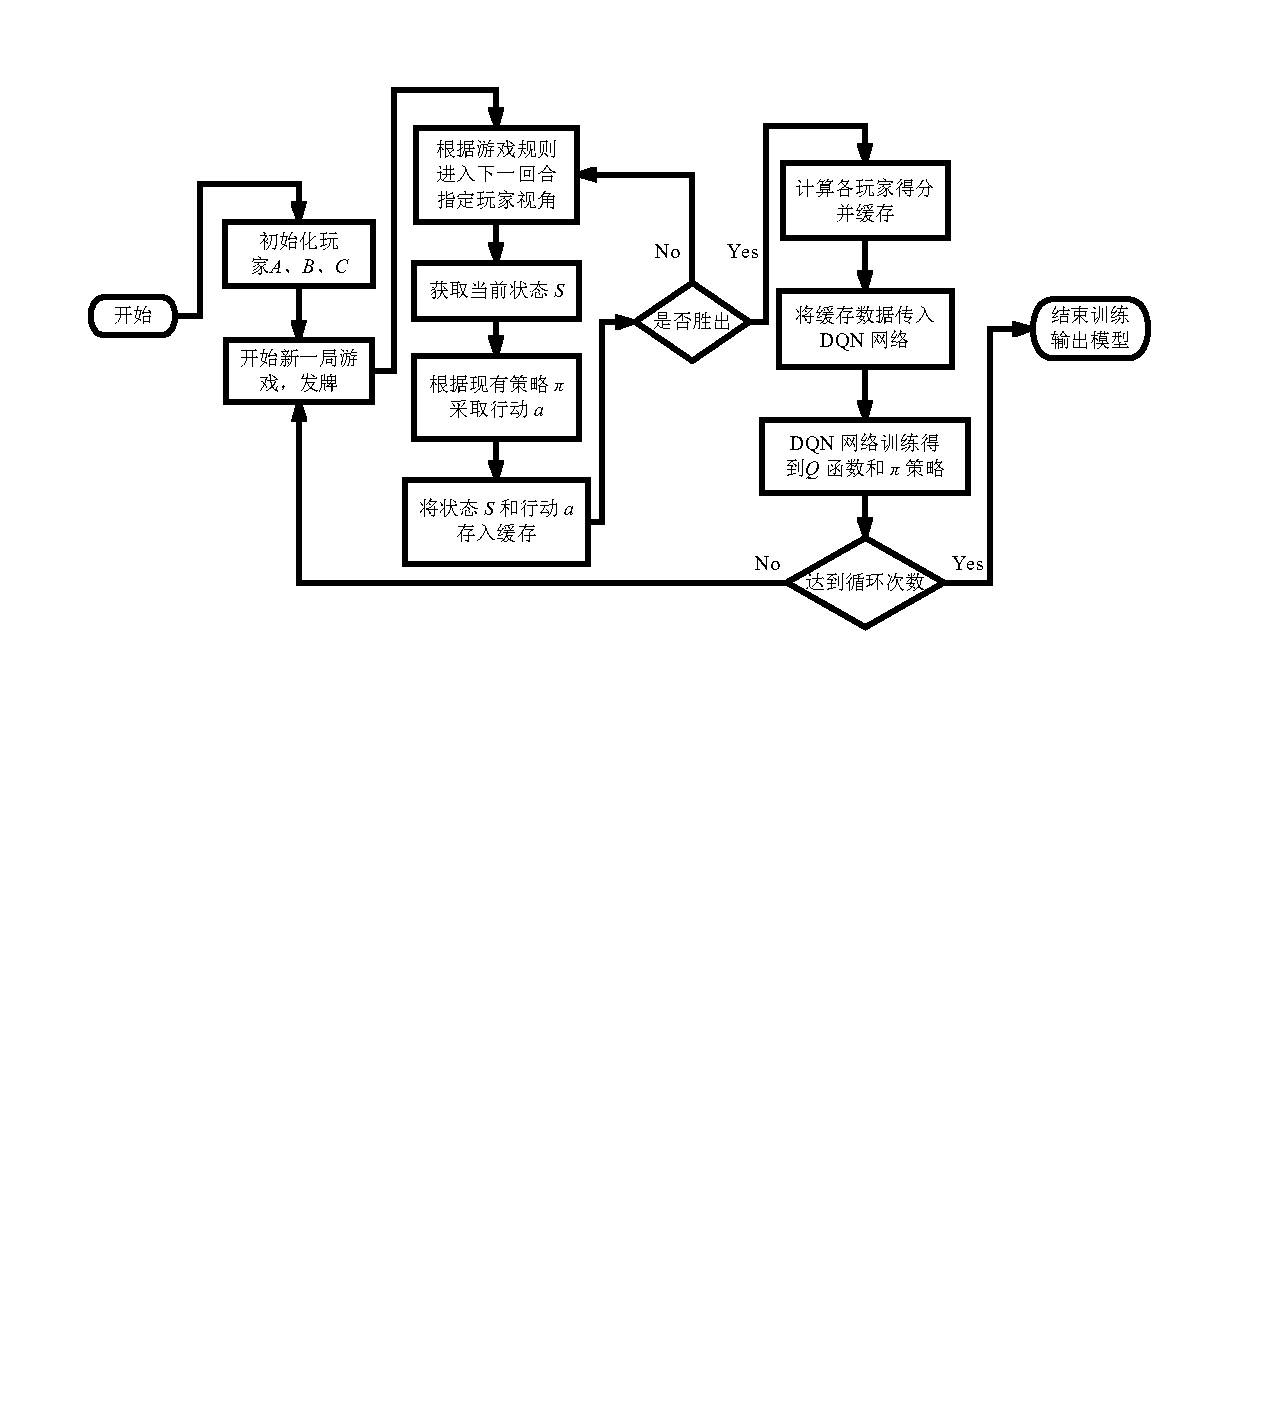
\includegraphics[width=\textwidth]{DQN-Process.pdf}
    \caption{实验流程图}
\end{figure}

\section{仿真实验结果与分析}

在自适应 Deep Q-Learning 算法中,

在 NVIDIA GTX 1080 GPU 的环境下,经过 50 万局自我对战学习(其中每 1000 局作为一个 epoch 集中学习),最终决策函数 $Q$ 得到收敛。

\begin{figure}[H]
    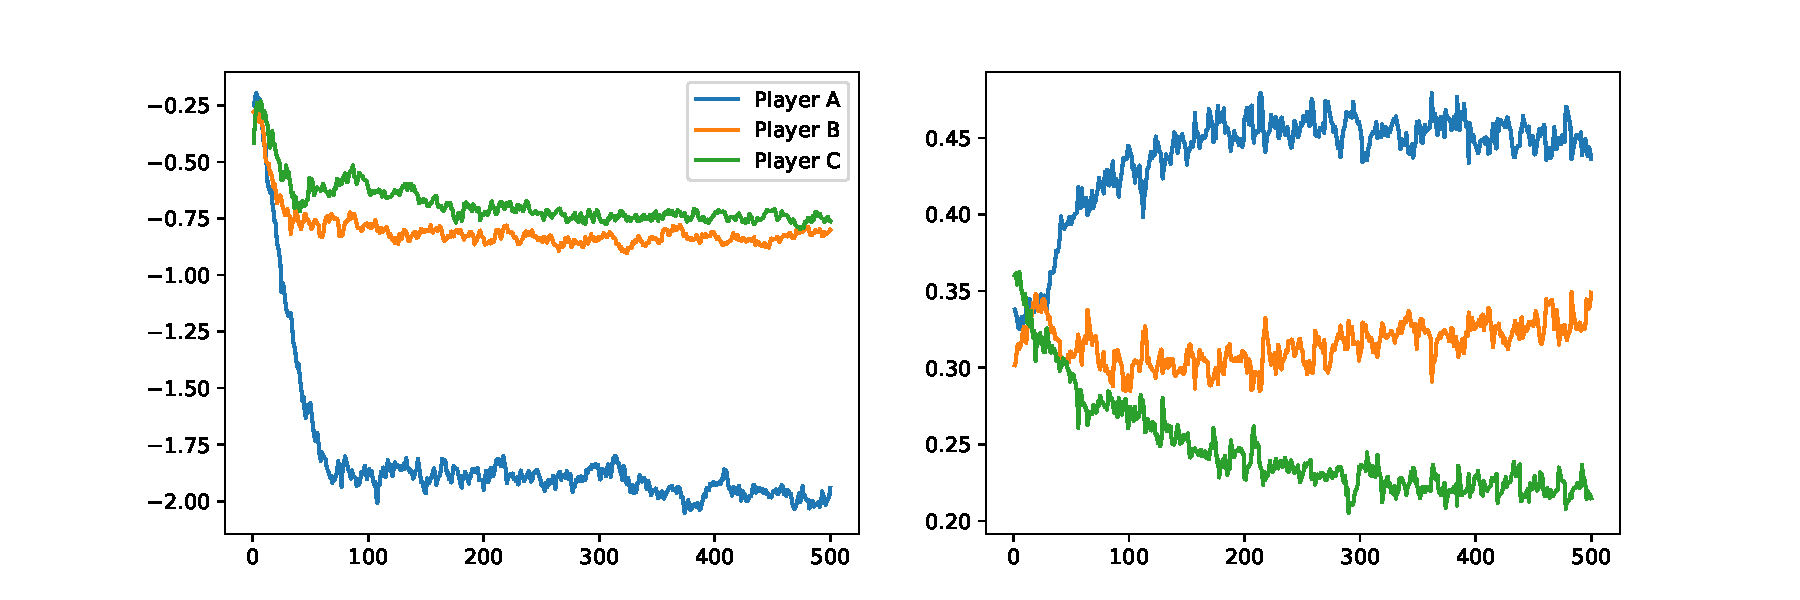
\includegraphics[width=\textwidth]{q-wr.pdf}
    \caption{Q 函数与实时训练胜率}\label{img:q-wr}
\end{figure}

从\ref{img:q-wr}的左图可以看出,经过自适应 Deep Q-Learning 算法训练可使行动价值函数 $Q(s,a)$ 收敛,进而可以得到 $\varepsilon$-贪心策略:

\begin{equation}
    \pi(a|s)=
    \begin{cases}
        \frac{\varepsilon}{|\mathcal A(s)|}&, a\neq\arg\max_aQ(s,a)\\
        1-\varepsilon-\frac{\varepsilon}{|\mathcal A(s)|}&, a=\arg\max_aQ(s,a)
    \end{cases}
\end{equation}

其中策略 $\pi(a|s)$ 是一个条件概率分布,其含义是模型处于状态 $s$ 时,决定采取行动 $a$ 的概率。

从\ref{img:q-wr}的右图可以观察发现,在训练过程中,最优算法模型的胜率不断上升并收敛,远优于另外两个普通的游戏模型,可以得知,自适应 Deep Q-Learning 算法确实通过强化学习的思想学习和掌握了一定的人类游戏技巧。

